\documentclass[12pt]{article}
\usepackage{HomeWorkTemplate}
\usepackage{circuitikz}
\usepackage[shortlabels]{enumitem}
\usepackage{hyperref}
\usepackage{tikz}
\usepackage{xepersian}
\usepackage{graphicx}
\usetikzlibrary{arrows,automata}
\usetikzlibrary{circuits.logic.US}
\settextfont{XB Niloofar.ttf}
\usepackage{changepage}
\newcounter{problemcounter}
\newcounter{subproblemcounter}
\setcounter{problemcounter}{1}
\setcounter{subproblemcounter}{1}
\newcommand{\problem}[1]
{
	\subsection*{
		پرسش
		\arabic{problemcounter} 
		\stepcounter{problemcounter}
		\setcounter{subproblemcounter}{1}
		#1
	}
}
\newcommand{\subproblem}{
	\textbf{\harfi{subproblemcounter})}\stepcounter{subproblemcounter}
}



\begin{document}

\handout
{نظریه زبان‌‌ها و اتوماتا}
{تمرین سری یک}
{امیررضا اکبری}
{۱۱۱۱۱۱۱۱}
{}
\problem{}
\subproblem{}
 به سادگی مشخص است که این عبارت غلط است زیرا شخصی که از این رستوران سفارش داده است یا از قبل سفارش داده بوده
 که به وضوح راضی بود و مشتری رستوران است و نظر ان مثبت و در غیر این صورت این شخص از طرف شخصی دیگر
 که سلیقه های مشابهی دارند معرفی شده یا خودش در نگاه اول از رستوران راضی بوده که این رستوران را برای سفارش انتخاب کرده
 و در کل تعداد حالات کمی وجود دارد که شخص نظر منفی داشته باشد و این نمونه گیری به وضوح اریب است.
\newline
\subproblem{} 
این نمونه گیری نیز به دلایل مختلفی که چند نمونه را ذکر خواهم کرد اریب است. یکی اینکه ریاضی دو درسی پایه و اجباری است.
یکی دیگر اینکه درس فلسفه ریاضی فقط مربوط به دانشکده ریاضی و همجین درس اختیاری است در صورتی که 
ریاضی دو مربوط به کل دانشگاه و اجباری است.
یکی دیگر از دلایل این است که برای خیلی از دانشجویان نمره خوب را به سادگی گرفتن ملاک است ولی دکتر شهشهانی استادی
سخت گیر است.
\problem{}
\subproblem{}
از لحاظ مفهومی چولگی به معنای میزان دوری داده های پرت است یا به عبارتی
علامت آن نشان دهنده راست یا چپ بودن داده های دور تر از میانگین یا مد است.
\newline
\subproblem{}
با توجه به ضریب چولگی اول پیرسن ($\frac{\bar{x} - M}{s} $) چپ بودن چولگی به معنای منفی بودن این عبارت و درنتیجه بزگ تر بودن مد از میانگین است.
\newline 
   منفی بودن این عبارت نشان دهنده بزرگ تر بودن میانه نسبت به میانگین است. ($\frac{3(\bar{x} - m)}{s} $) از طرف دیگر با توجه به ضریب چولگی دوم پیرسن 
\newline
  پس کافیست نشان دهیم رابطه بین مد و میانه چگونه است از طرف دیگر با توجه به ضریب چولگی گشتاوری منفی بودن چولگی به معنی وجود داده بیشتر داده های دور تر از میانگین در سمت چپ میانگین است که
این به معنی بزرگ تر بودن بازه 
\newline
\subproblem{}
برابر بودن ضریب اول و دوم پیرسن به ما رابطه زیر را می دهنده
\newline
$\frac{\bar{x} - M}{s} $ = $\frac{3(\bar{x} - m)}{s} $ = 0.32
\newline
 که با قرار دادن میانگین و انحراف معیار به ترتیب داریم:
 \newline
 $\frac{29.6 - M}{6.5} = 0.32 $\newline
 $ M = 27.52$ : مد
 \newline
 $\frac{3(29.6 - m)}{6.5} = 0.32 $\newline
 $29.6 - m = 0.693$\newline
 $m = 28.9 $ تقریباااااا
\problem{}
\subproblem{}
\begin{figure}[h]
	\centering
	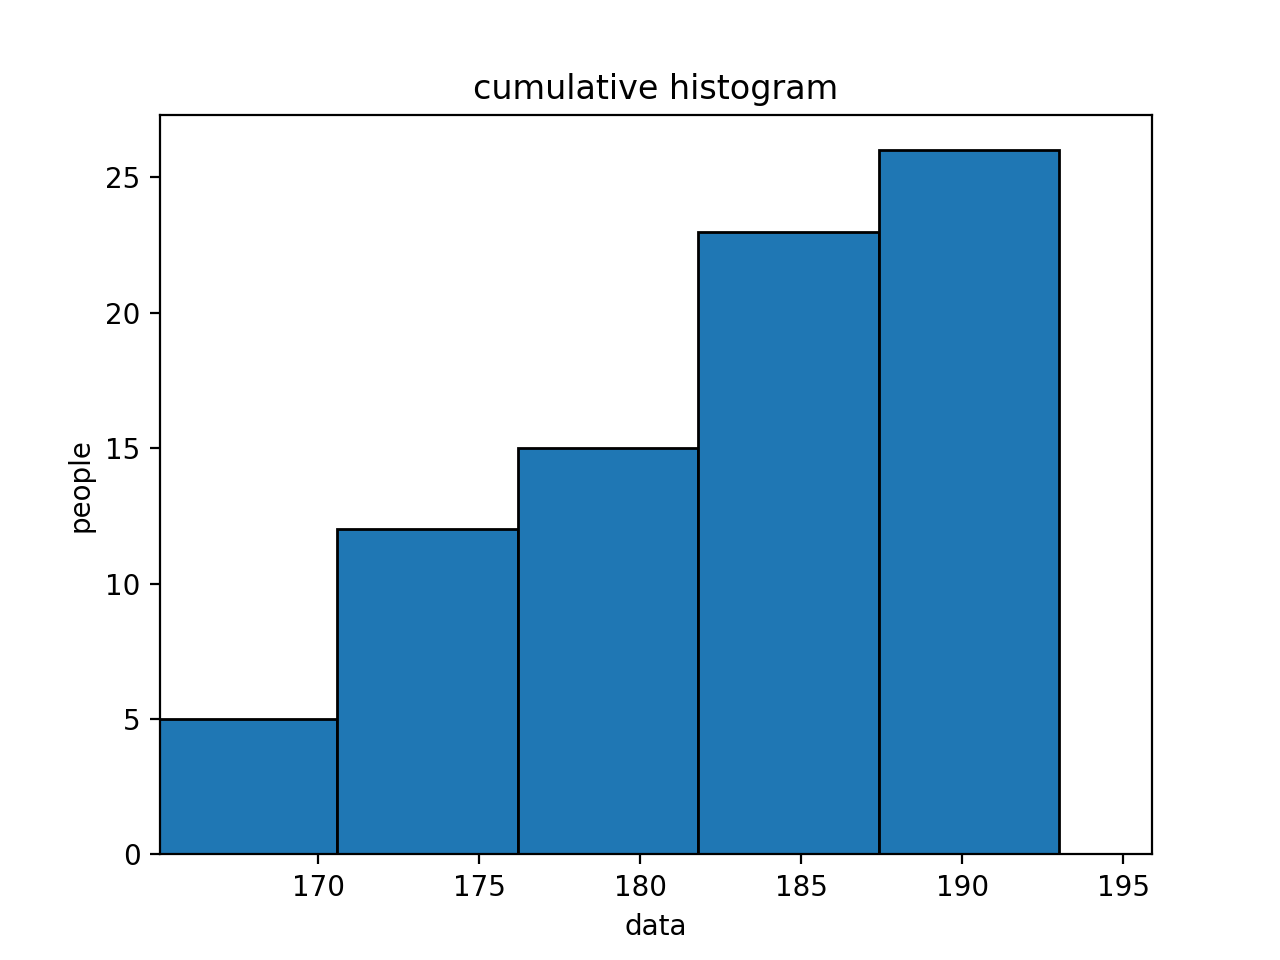
\includegraphics[width=0.5\textwidth]{Figure_1.png}
	\caption{نمودار توزیع تجمعی رسم شده توسط python}
\end{figure}

\subproblem{}
برای به دست اوردن میانگین کافیست مقدار مرکز دسته ها را محاسبه کنیم و برای هر دسته مقدار مرکز دسته را در فراوانی نسبی دسته
ضرب کنیم و در نهایت با هم جمع کنیم.
\newline
\newline
$\bar{X} = \frac{4 * 167.5 + 5 * 172.5 + 3 * 177.5 + 7 * 182.5 + 5 * 187.5 + 2 * 192.5}{26} = 179.423$
\newline
\newline
حالا برای پیدا کردن میانه کافیست با ببینیم در نمودار کدام دسته است که دسته قبل از آن کمتر از ۱۳ و دسته بعد از آن بیشتر از ۱۳ فراوانی تجمعی دارد.
که با توجه به شکل دسته ۱۸۰ تا ۱۸۵ دسته مورد نظر ماست که ابتدای دسته ۱۲ و انتهای آن ۱۹ است و با قضیه تالس به سادگی مشخص میشود که اگر یک خط از نقطه (180,12) و (185,19) رد کنیم
در نقطه ۱۸۰ + ۵/۷ یعنی تقریبا 180.71 میانه ما به دست می آید.
که نسبت تالس به صورت زیر است:\newline
\begin{figure}[]
	\centering
	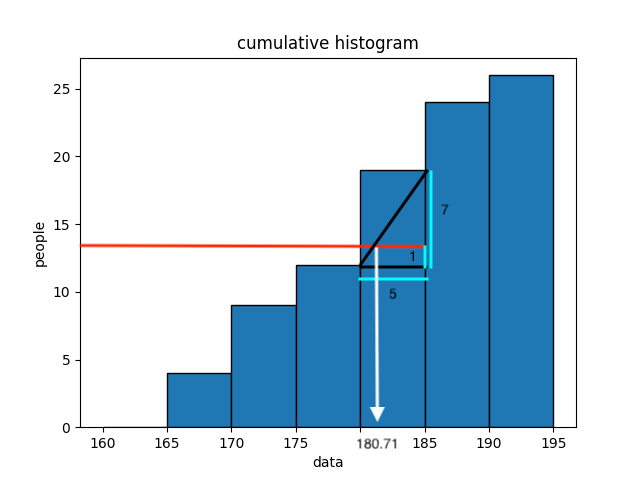
\includegraphics[width=0.5\textwidth]{Figure_4.png}
	\caption{پیدا کردن میانه در نمودار هیستوگرام به کمک روش تالس}
\end{figure}

\problem{}

\subproblem{}
کافیست یک مثال نقض از توزیعی بیاورم که میانگین آن (که برای توزیع پیوسته به صورت امید ریاضی تعریف میشود)
جایی باشد که تابع توزیع آن برابر با یک دوم نشود.
برای مثال در شکل زیر تنها نقطه ای که F(x) برای آن برابر با
یک دوم میشود صفر است اما به وضوح امید ریاضی یا همان میانگین این نمودار بزرگ تر از صفر است.

\begin{figure}[]
	\centering
	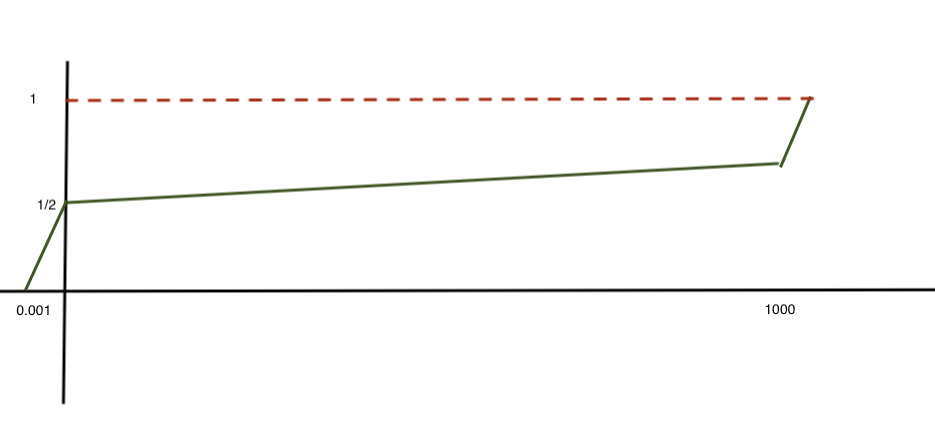
\includegraphics[width=0.5\textwidth]{Figure_5.png}
	\caption{مثال نقض برای قسمت آ سوال چهار}
\end{figure}

\subproblem{}
اگر میانه توزیع را برای حالت پیوسته تعریف کنیم نقطه ای در تابع چگالی که در آن انتگرال قبل و بعد از أن
برابر با یک دوم میشود این دقیقا تعریفی هست که در صورت سوال گفته شده و میانه در آن می افتد.
\newline
\subproblem{}
برای این قسمت کافیست یک توزیع نامتقارن ارایه دهیم که هر دوی میانه و میانگین عوض این مجموعه باشند.

\problem{}

\[ e = P(E) \]
\[ f = P(F) \]
\[ s = P((F \cup E)^{c}) = 1 - e - f \]

با تعریف احتمالات بالا و فرض مستقل بودن آزمایش‌ها، احتمال رخ دادن E قبل از F برابر است با مجموع تمام حالت‌هایی که مجموعه‌ای ازمایش رخ داده و نه F و نه E رخ داده است و در آخرین آزمایش E رخ داده است. از آنجایی که این پیشامد‌ها اشتراکی ندارند، احتمال اجتماع آنها جمع احتمالاتشان است. بنابراین:

\[ P(E \text{ قبل } F) = \sum_{i=0}^{n} (s^i \times e) = e \times \sum_{i=0}^{n} (s^i) \]

که یک سری هندسی است و جمع آن به صورت زیر حساب می‌شود:

\[ \lim_{n \to \infty} \left( \frac{(1 - (s^n))}{1 - s} \right) = \frac{1}{1 - 1 + e + f} \]

در نتیجه داریم:

\[ P(E \text{ قبل } F) = \frac{e}{f+e} = \frac{P(E)}{P(E)+P(F)} \]
\problem{}
\end{document}